\documentclass[11pt]{article}

\usepackage{fancyhdr}
\pagestyle{fancy}
\newcommand\course{ASTR 102}
\newcommand\hwnumber{3}
\newcommand\duedate{October 20, 2020}

\lhead{Oliver Tonnesen\\V00885732}
\chead{\textbf{\Large Lab \hwnumber{} Report}}
\rhead{\course\\\duedate}

\usepackage[
	backend=biber,
	url=true
]{biblatex}
\addbibresource{lab3.bib}
\usepackage{enumitem}
\usepackage{graphicx}
\usepackage{url}
\usepackage{pgfplots}
\pgfplotsset{width=10cm,compat=1.9}

\usepackage{amssymb}

\usepackage{pdflscape}


\begin{document}
\section{Objective}
In this lab we explore the creation, interpretation, and parameters of the colour-magnitude diagram (CMD).
Additionally, we see some applications of the CMD, specifically with respect to determining the age, distance, and dust reddening of open clusters.


\section{Introduction}
Clusters of stars generally form together, so we can assume all the stars in any given cluster share the same age, composition, and distance from Earth.
That isn't to say that all the stars in a cluster are all the same; a cluster's stars will often vary significantly in both mass and colour.

These two properties prove very useful in studying star clusters.
The tool we use to study these properties in a star cluster is the colour-magnitude diagram (CMD), which plots magnitude against colour.
To measure a star's brightness, we measure its apparent magnitude through a yellow filter.
This is called the star's $V$-band brightness.
To measure its colour, we measure its brightness again -- this time through a blue filter -- and take the difference of this with its brightness through the yellow filter.
This is called the star's $(B - V)$ colour.

Plotting these values onto a CMD, we can extract quite a bit of information about the star cluster as a whole.
For example, an abundance of bright, blue stars likely means that a star cluster is young, since blue stars have relatively short lifespans.
Conversely, if we see mostly faint, red stars, we can deduce that the brightest and most massive stars have all died off, and that the star cluster is relatively old.

Colour-magnitude diagrams are affected by two principal factors: \emph{distance} and \emph{dust reddening}.
The first factor affecting the CMD, distance, is quite intuitive: the further a star cluster is from Earth, the fainter its stars will appear.
We can account for this by considering the difference between a star's apparent ($m$) and absolute ($M$) magnitude, called its \emph{distance modulus}, $\mu = m - M$.
It's important to note that a star's distance from us affects only its apparent magnitude, and does not affect its colour.
The other factor affecting the CMD is dust reddening: as light from distant stars travels to us, it passes through interstellar dust.
Shorter wavelengths of light are much more likely to be absorbed by this interstellar dust, and so stars appear more red as their light passes through more dust.
We use the following equation (for clusters in the Milky Way) to correct for dust reddening:
\[mv_{corr} = mv_{obs} - 3.1 \times E(B - V)\]
where $mv_{corr}$ is our corrected magnitude, $mv_{obs}$ is our observed magnitude, and $E(B - V)$ is the \emph{colour excess}, roughly the "amount" of reddening we observe.


\section{Observations, Tables, and Graphs}

\begin{landscape}
\begin{table}[h]
\caption{Observed features in the CMD of clusters.}
\begin{tabular}{| c | c | c | c | c | c | c | p{11cm} |}
	\hline
	Cluster & MS & TO & SG & RG & HB & BS & Comments \\ \hline
	M 15 & $\checkmark$ & $\checkmark$ & $\checkmark$ & $\checkmark$ & $\checkmark$ & $\checkmark$ & The horizontal branch appears attached to the blue stragglers, it's hard to say if what might be the blue stragglers is actually just an extension of the horizontal branch. \\ \hline
	NGC 6791 & $\checkmark$ & $\checkmark$ & $\checkmark$ & $\checkmark$ & $\times$ & $\times$ & The main sequence is all over the place, and the blue stragglers are hard to make out through all the noise around the main sequence. \\ \hline
	NGC 104 & $\checkmark$ & $\checkmark$ & $\checkmark$ & $\checkmark$ & $\checkmark$ & $\times$ & This cluster has very defined features for the most part. There are a few stars above and to the left of the turn off, but not enough to call it a feature of the cluster. \\ \hline
	NGC 188& $\checkmark$ & $\checkmark$ & $\checkmark$ & $\checkmark$ & $\times$ & $\checkmark$ & This cluster has a very faint red giant branch, just barely enough to really say it has one at all. \\ \hline
	M 67 & $\checkmark$ & $\checkmark$ & $\checkmark$ & $\checkmark$ & $\times$ & $\checkmark$ & The red giant branch is not very defined at all, and the main sequence is also very fuzzy. \\ \hline
	NGC 6819 & $\checkmark$ & $\checkmark$ & $\times$ & $\times$ & $\times$ & $\checkmark$ & No discernible sub-giant or red giant branch. Quite a few blue stragglers. \\ \hline
	Hyades & $\checkmark$ & $\times$ & $\times$ & $\times$ & $\times$ & $\times$ & This cluster is very bright; its brightest stars have magnitude 5. No discernible features other than main sequence. Could possibly have blue stragglers, but very hard to say without turn off. \\ \hline
	Praesepe & $\checkmark$ & $\times$ & $\times$ & $\times$ & $\times$ & $\checkmark$ & Another bright cluster. Similar to Hyades, but the blue stragglers are quite a bit more defined. \\ \hline
	Pleiades & $\checkmark$ & $\checkmark$ & $\times$ & $\times$ & $\times$ & $\times$ & There does appear to be a turn off in this cluster, but it is much bluer than the turn offs in all the other clusters so far. Otherwise no distinctive features. \\ \hline
	NGC 6611 & $\checkmark$ & $\times$ & $\times$ & $\times$ & $\times$ & $\times$ & The only feature this cluster appears to have it a main sequence consisting entirely of very bright, blue stars. \\ \hline
	h+x Perseii & $\checkmark$ & $\checkmark$ & $\times$ & $\times$ & $\times$ & $\times$ & This is another cluster of very blue stars. What seems to be a turn off point is starting to appear above the main sequence. \\ \hline
	Hipparcos & $\checkmark$ & $\checkmark$ & $\checkmark$ & $\times$ & $\times$ & $\checkmark$ & This cluster has a very large number of incredibly bright blue stars. What would appear to be the blue stragglers is as densely packed as the main sequence itself, making the turn off point very hard to distinguish. There is a sub-giant branch, but no red giant branch. \\
	\hline
\end{tabular}
\label{table:CMD_Features}
\end{table}
\end{landscape}

\begin{table}[h]
\caption{Distances to clusters from Sun's magnitude.}
\begin{tabular}{| c | c | c | c | c |}
	\hline
	Cluster name & Sun's V-mag & Visible? (Y/N) & Distance modulus, $\mu$ & Distance d [pc] \\ \hline
	Hyades & $8.0 \pm 1.0$ & N & 3.0 & 39 \\ \hline
	Praesepe & $10.8 \pm 0.7$ & N & 5.8 & 140 \\ \hline
	Pleiades & $10.3 \pm 0.8$ & N & 5.3 & 110 \\ \hline
	NGC 188 & $15.4 \pm 4.1$ & N & 10.4 & 1200 \\ \hline
	M 15 & $21.3 \pm 0.5$ & N & 16.3 & 18000 \\
	\hline
\end{tabular}
\label{table:CMD_distances}
\end{table}

\begin{figure}[h]
\caption{Hertzsprung-Russel Diagram for M 67}
\center
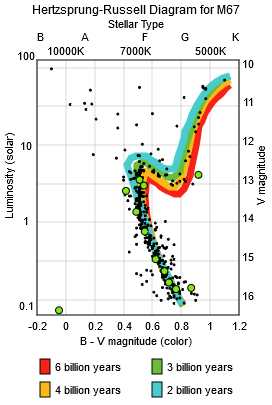
\includegraphics[scale=0.5]{figures/hr.jpg}
\label{fig:hr-m67}
\end{figure}


\section{Answers}
\begin{enumerate}[label={\textbf{\emph{(\arabic*)}}}]
	\item % 1
Please see Table~\ref{table:CMD_Features}.
	\item % 2
Please see Table~\ref{table:CMD_distances}.
	\item % 3
Please see Table~\ref{table:CMD_distances}.
	\item % 4
None of the distance moduli we calculated were negative, so since we're assuming that the distance scales linearly with the distance modulus, we can conclude that none of the clusters are closer to us than 10 parsecs.
	\item % 5
The cluster for which the Sun had the smallest distance modulus was Hyades, with $\mu = 3$.
Plugging this value for $\mu$ into $d = 10^{0.2\mu + 1}$ gives us distance $d \approx 39$.
All other clusters are at least this far, so none of them are within 10 parsecs of us.
	\item % 6
Based on our calculations, Hyades, Praesepe, and Pleiades should be closer than 8000 pc.
None of them should be further than 30 000 pc.
The furthest should be M 15, at around 18 200 pc.
	\item % 7
Decreasing the age shifts the isochrone to the left on the plot, and increasing it shifts the isochrone to the right.
Earlier in the cluster's lifespan, there should be more young, blue stars.
These blue stars die off much quick than the cooler red stars, which is why as the age of the cluster is increased, the line fitting the stars moves to the right, becoming more red as more blue stars die off and more main sequence stars become red giants.
	\item % 8
Decreasing the distance modulus shifts the isochrone up on the plot, and increasing it shifts the isochrone down.
A decrease in distance modulus means a decrease in apparent magnitude or an increase in absolute magnitude.
If we assume, on average, that any two star clusters might have a similar amount of stars of a given absolute magnitude, then we would expect lowering the distance modulus to result in a lower apparent magnitude.
Similarly, we would expect raising the distance modulus to result in a high apparent magnitude.
	\item % 9
A decrease in distance modulus means a decrease in apparent magnitude or an increase in absolute magnitude.
If we assume, on average, that any two star clusters might have a similar amount of stars of a given absolute magnitude, then we would expect lowering the distance modulus to result in a lower apparent magnitude.
Similarly, we would expect raising the distance modulus to result in a high apparent magnitude.
	\item % 10
M 67 is one of the oldest star clusters in the sky.
Its age is estimated to be $3.5 \pm 0.5$ billion years, and its distance is estimated to be between 800 and 900 parsecs.
M 67 is estimated to contain around 500 stars, many of which belong to its significant main sequence and red giant branches \cite{seds-m67}.
One particularly interesting characteristic about this cluster that its age is very close to that of our Solar System, and as such many of its main sequence stars share similar characteristics (such as size and chemical composition) to the Sun.
	\item % 11
Based on the isochrone fit using the online tool (see Figure~\ref{fig:hr-m67}), we estimate M 67 to be approximately 3 billion years old.
This is indeed within the expected uncertainty.
	\item % 12
M 67's colour-magnitude diagram has a pronounced turn off and red giant branch.
The vast majority of its stars are red in colour, and a lot of them are still in main sequence.
This seems to imply that M 67 is indeed quite old, as most of its blue stars appear to have died off, leaving mostly dim red stars.
This leads us to believe that our estimate of 3 billion years was reasonably accurate.
\end{enumerate}


\section{Discussion}
This lab exercise demonstrated how to create and read colour-magnitude diagrams.
We saw how to locate some different features of the colour-magnitude diagram, such as main sequence, blue stragglers, and red giants, and how to interpret the presence or absence of these features with respect to a star cluster's age, distance.

There were lots of places for error and uncertainty in this lab.
The main source of our uncertainty was in estimating the distance of faraway star clusters: we tried to insert our Sun into the main sequence branch of a star cluster's CMD, and from this determine the distance modulus.
It's hard to say where exactly in the main sequence the Sun would actually be, since in some cases, the star cluster's main sequence branch was as thick as 4.1 magnitude.
Some other, more minor sources of error and uncertainty were in the measuring of a star's apparent magnitude from an image and using a chart to convert from distance modulus to distance in parsecs instead of using the formula directly.
Additionally, we did not account for the metallicity and chemical composition of the star clusters, so we might have missed out on any insight those properties may have provided.


\section{Conclusion}
In this lab exercise, we learned how to interpret colour-magnitude diagrams, and how they are affected by variables such as distance, age, and dust reddening.
We learned about some applications of colour-magnitude diagrams, particularly in the estimation of the age and distance of star clusters.
We also saw how colour-magnitude diagrams can be created directly by measuring the apparent magnitudes of many stars in a cluster and compiling them into a single graph.


\printbibliography

\end{document}
